% Source: Code/RADAR_web/docs/figures/fig_modules.tex
\documentclass[border=5pt]{standalone}
\usepackage{tikz}
\usetikzlibrary{arrows.meta,positioning}
\usepackage{xcolor}

\definecolor{garnet}{HTML}{73000A}
\definecolor{black10}{HTML}{ECECEC}
\definecolor{atlantic}{HTML}{466A9F}

\begin{document}
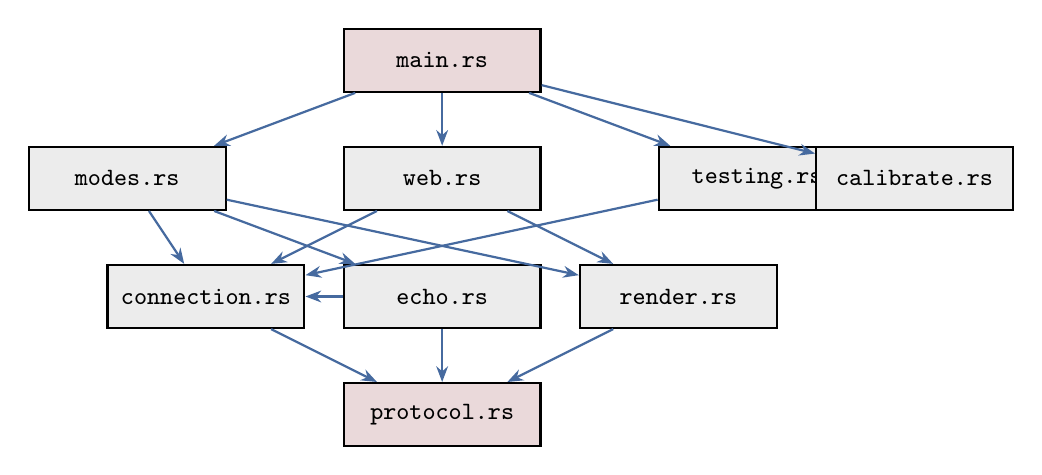
\begin{tikzpicture}[
    mod/.style={draw, thick, minimum width=2.5cm, minimum height=0.8cm, align=center, fill=black10, font=\ttfamily\small},
    dep/.style={-{Stealth[length=2mm]}, thick, color=atlantic},
]

\node[mod, fill=garnet!15] (main) at (0, 3) {main.rs};
\node[mod] (modes) at (-4, 1.5) {modes.rs};
\node[mod] (web) at (0, 1.5) {web.rs};
\node[mod] (testing) at (4, 1.5) {testing.rs};
\node[mod] (calibrate) at (6, 1.5) {calibrate.rs};
\node[mod] (connection) at (-3, 0) {connection.rs};
\node[mod] (echo) at (0, 0) {echo.rs};
\node[mod] (render) at (3, 0) {render.rs};
\node[mod, fill=garnet!15] (protocol) at (0, -1.5) {protocol.rs};

\draw[dep] (main) -- (modes);
\draw[dep] (main) -- (web);
\draw[dep] (main) -- (testing);
\draw[dep] (main) -- (calibrate);
\draw[dep] (modes) -- (connection);
\draw[dep] (modes) -- (echo);
\draw[dep] (modes) -- (render);
\draw[dep] (web) -- (connection);
\draw[dep] (web) -- (render);
\draw[dep] (testing) -- (connection);
\draw[dep] (echo) -- (protocol);
\draw[dep] (connection) -- (protocol);
\draw[dep] (render) -- (protocol);
\draw[dep] (echo) -- (connection);

\end{tikzpicture}
\end{document}
